\chapter{Mengen}
\section{Definitionen}
\subsection{Definition von Mengen}
Eine Menge\index{Menge} ist eine Zusammenfassung von wohl unterscheidbaren Objekten\index{Objekt}. Diese Objekte hei�en Elemente der Menge.
Man bezeichnet Mengen normalerweise mit gro�en lateinischen Buchstaben.
\[ \mathbb{A}, \mathbb{B}, \mathbb{C} \]
Ist $M$ eine Menge und $x$ ein Objekt so scheiben wir $x \in M$, falls $x$ in $M$ enthalten ist und $x \notin M$, falls $x$ nicht in $M$ enthalten ist.\\
Es muss eindeutig feststellbar sein, ob das Objekt $x$ Element von $M$ ist oder nicht.\\
Eine Menge kann auf verschiedene Arten beschrieben werden.
\begin{enumerate}
	\item durch Aufz�hlung z.B.:\\$A := $\gklamm{\mbox{rot; gelb; blau}}\\$B := $\gklamm{\mbox{Regensburg; M�nchen; Bonn}}\\$C := $\gklamm{1; 3; 5; 7}\\\\Hierbei bedeutet $:=$ das die linke Seite durch die rechte Seite definiert wird.\\$...$ darf nur geschrieben werden, wenn eindeutig klar ist, was damit gemeint ist.
	\item durch die Angabe von Eigenschaften welche die Menge charakterisieren\\$D := $\gklamm{x|x \mbox{ ist durch } 2 \mbox{ teilbar}}\\$E := $\gklamm{x|x \mbox{ ist eine deutsche Stadt}}\\$F := $\gklamm{x|x > -5}
\end{enumerate}

\subsubsection{Beispiele f�r bekannte Mengen}
\begin{itemize}
	\item \textfakealign{$\mathbb{N}_0$}{$\mathbb{N}$}{$:= \gklamm{1; 2; 3; 4; 5;\dots} = $ Menge der nat�rlichen Zahlen\index{Nat�rliche Zahlen $\mathbb{N}$}}
	\item \textfakealign{$\mathbb{N}_0$}{$\mathbb{N}_0$}{$:= \gklamm{0; 1; 2; 3; 4;\dots} = $ Menge der nat�rlichen Zahlen mit $0$\index{Nat�rliche Zahlen $\mathbb{N}$!Mit Null $\mathbb{N}_0$}}
	\item \textfakealign{$\mathbb{N}_0$}{$\mathbb{Z}$}{$:= \left\{0; 1; -1; 2; -2; 3; -3;\dots \right\}$\index{Ganze Zahlen $\mathbb{N}$}\\
		   $:= \left\{\dots; -3; -2; -1; 0; 1; 2; 3 \right\} = \mbox{ Menge der ganzen Zahlen}$}
	\item \textfakealign{$\mathbb{N}_0$}{$\mathbb{Q}$}{$ := \gklamm{x|x = \frac{a}{b}, a \in \mathbb{Z}, b \in \mathbb {N}} =$ Menge der rationalen Zahlen\index{Rationale Zahlen $\mathbb{Q}$}}
	\item \textfakealign{$\mathbb{N}_0$}{$\mathbb{R}$}{$=$ Menge der reellen Zahlen\index{Reelle Zahlen $\mathbb{R}$}}
\end{itemize}

\subsection{Definition der leeren Menge}
Nach der Definition der Mengen gibt es genau eine Menge die kein Objekt enth�lt.
Diese Menge nennt man leere Menge und bezeichnet sie mit $\{\}$ oder $\emptyset$.\index{Leere Menge $\emptyset$, $\{\}$}

\subsection{Definition echter Teil- oder Obermengen}
Eine Menge $B$ hei�t Teilmenge\index{Teilmenge $\subseteq$} von $A$ (bezeichnet mit $B \subseteq A$), falls jedes Element von $B$ auch Element von $A$ ist.\\
Eine Menge $B$ hei�t echte Teilmenge\index{Echte Teilmenge $\subset$} von $A$ (bezeichnet mit $B \subset A$), falls $B$ Teilmenge von $A$ ist und es existiert ein Element $y$ aus $A$, das nicht in $B$ enthalten ist.\\
Wenn $B$ (echte) Teilmenge von $A$ ist bezeichnet man $A$ als (echte) Obermenge\index{Echte Obermenge $\supseteq$}\index{Obermenge $\supset$} von $B$, in Zeichen $A \supseteq B$ bzw. $A \supset B$.\\
\textalign{Beispiel:}{$\mathbb{N} \subset \mathbb{N}_0 \subset \mathbb{Z} \subset \mathbb{Q} \subset \mathbb{R}$}

\subsection{Definition von Mengenoperatoren}
Seien $A$ und $B$ beliebige Mengen und $M \supset A$.
\begin{enumerate}
\item Der Durchschnitt\index{Durchschnitt $\cap$} oder Schnitt\index{Schnitt $\cap$} ($A \cap B$) von $A$ und $B$ ist die Menge\[A \cap B := \left\{x|x \in A \mbox{ und } x \in B\right\}\] $A \cap B$ enth�lt alle Elemente, die sowohl in $A$ als auch in $B$ enthalten sind.\\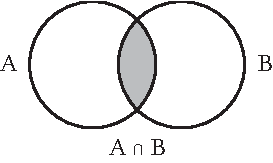
\includegraphics{bilder/kapitel/kap1_Mengen/1.pdf}%IMG-02.10.2008-mathe-1
\item Die Vereinigung\index{Vereinigung $\cup$} $A \cup B$ von $A$und $B$ die Menge\[A \cup B := \left\{x|x \in A \mbox{ oder } x \in B\right\}\] $A \cup B$ enth�lt also alle Elemente die in mindestens einer der beiden Mengen A und B enthalten ist.\\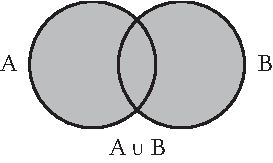
\includegraphics{bilder/kapitel/kap1_Mengen/2.pdf}%IMG-02.10.2008-mathe-2
\item Die Differenz\index{Differenz $\backslash$} ($A \backslash B$) von $A$ und $B$ ($A \backslash B$ spricht man auch ''$A$ ohne $B$'' oder ''$A$ minus $B$'')\[A \backslash B := \left\{x|x \in A \mbox{ und } x \notin B\right\}\] daher $A \backslash B$ enth�lt alle Elemente aus $A$ die nicht in Element von $B$ sind.\\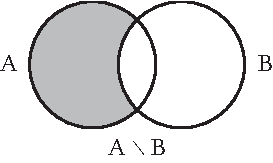
\includegraphics{bilder/kapitel/kap1_Mengen/3.pdf}%IMG-02.10.2008-mathe-3
\item Die symmetrische Differenz\index{Symmetrische Differenz $\triangle$} $A \triangle B$ von $A$ und $B$ ist die Menge\[A \triangle B := (A \backslash B) \cup (B \backslash A)\] $A \triangle B$ enth�lt alle Elemente, die entweder in $A$ oder in $B$ enthalten sind (ausschlie�endes oder), bzw. alle Elemente, die in genau einer der Mengen $A$ oder $B$ enthalten sind.\\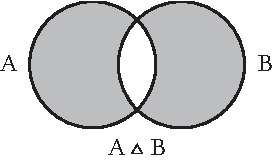
\includegraphics{bilder/kapitel/kap1_Mengen/4.pdf}%IMG-06.10.2008-mathe-1
\item Das Komplement\index{Komplement $\overline{M}$} $\overline{A}$ (bzw. $A^c$) von $A$ bez�glich $M$ ist die Menge\[\overline{A} := M \backslash A = \left\{ x \in M | x \notin A \right\}\] $A$ enth�lt alle Elemente aus $M$, die nicht in $A$ enthalten sind.
\item Die Produktmenge\index{Produktmenge $\times$} $A \times B$ (oder kartesisches Produkt) der Mengen $A$ und $B$ ist die Menge\[A \times B := \left\{ (a, b) | a \in A, b \in B \right\}\] $A \times B$ ist die Menge der geordneten Paare von Elementen aus $A$ und $B$.\\\\
		\textalign{Beispiel:}{
		$A = \{1,2\}, B = \{1\}$\\
		$A \times B =\{(1,1),(2,1)\}$\\
		$B \times A =\{(1,1),(1,2)\}$}
\end{enumerate}

\textalignmize{Bemerkung:}{}{
	\item Die in der Definition verwendeten Bildchen nennt man Venn-Diagramme\index{Venn-Diagramm}.
	\item Die Mengenoperationen $\cap$, $\cup$, $\triangle$ sind symmetrisch.
	\item Die Mengenoperation $A \times B$ ist nicht symmetrisch.}

\subsection{Weiter Definitionen}
\begin{enumerate}
\item Die Mengen $A$ und $B$ hei�en disjunkt\index{Disjunkt} falls $A \cap B = \emptyset$
\item F�r den Durchschnitt der Mengen $A_1$, $A_2$, $A_n$ schreibt man\[A_1 \cap A_2 \cap A_3 \cap \dots A_n = \bigcap_{k = 1}^n A_k\]
\item F�r die Vereinigung der Mengen $A_1$, $A_2$, $A_n$ schreibt man\[A_1 \cup A_2 \cup A_3 \cup \dots A_n = \bigcup_{k = 1}^n A_k\]
\item Ist $M$ eine endliche oder abz�hlbar unendliche Menge (z.B. $\mathbb{N}, \mathbb{Z}, \mathbb{Q}$), so hei�t die Menge aller Teilmengen von $M$ die Potenzmenge $\mathscr{P} (M)$ von $M$.\\Hat $M$ genau $m$ Elemente ($\betrag{M} = \# M = m$) so enth�lt die Potenzmenge\index{Potenzmenge} $\mathscr{P} (M)$ genau $2^m$ Elemente.\\\\
		\textalign{Beispiel:}{\vspace{-0.8em}
		$\begin{array}{lcl}
		M &=& \left\{0; 1; 2\right\}\\
		\mathscr{P} (M) &=& \left\{ \{0\}, \{1\}, \{2\}, \{0;1\}, \{0;2\}, \{1;2\}, \{0;1;2\}, \emptyset \right\}
		\end{array}$}

		\textalign{Beispiel f�r $\mathbb{N}$:}{
		$\mathscr{P} (\mathbb{N}) = \left\{\emptyset, \{1\}, \{2\}, \{3\}, \{1,2\}, \{1,3\}, \dots \right\}$}

\item Es muss beachtet werden das $\{ \emptyset \} \mbox{ oder } \left\{ \{ \} \right\} \neq \emptyset$
\item Falls $A \cap B = \emptyset$, $A, B$ endlich dann gilt\[\betrag{A \cup B} = \betrag{A} + \betrag{B}\]
\item Falls $B \subseteq A$, $A, B$ endlich dann gilt\[\betrag{A \backslash B} = \betrag{A} - \betrag{B}\]
\end{enumerate}

\section{\texorpdfstring{Rechenregeln f�r $\cap$, $\cup$ und $\overline{M}$}{Rechenregeln f�r Schnitt, Vereinigung und Negation}}
Sei $M$ eine Menge und $A, B, C \subseteq M$, so gelten folgende Rechenregeln:
\subsection{Assoziativgesetz}
\index{Mengen!Assoziativgesetz}
\begin{enumerate}
\item $(A\cap B)\cap C=A\cap(B\cap C)$
\item $(A\cup B)\cup C=A\cup(B\cup C)$
\end{enumerate}

\subsection{Distributivgesetz}
\index{Mengen!Distributivgesetz}
\begin{enumerate}
\item $A\cap(B\cup C)=(A\cap B)\cup(A\cap C)$
\item $A\cup(B\cap C)=(A\cup B)\cap(A\cup C)$
\item $(A\cup B)\cap C=(A\cap C)\cup(B\cap C)$
\item $(A\cap B)\cup C=(A\cup C)\cap(B\cup C)$
\end{enumerate}

\subsection{Kommutativgesetz}
\index{Mengen!Kommutativgesetz}
\begin{enumerate}
\item $A\cap B=B\cap A$
\item $A\cup B=B\cup A$
\end{enumerate}

\subsection{Idempotenzgesetz}
\index{Mengen!Idempotenzgesetz}
\begin{enumerate}
\item $A\cap A=A$
\item $A\cup A=A$
\end{enumerate}

\subsection{Absorptionsgestz}
\index{Mengen!Absorptionsgestz}
\begin{enumerate}
\item $A\cap(B\cup A)=A$
\item $A\cup(B\cap A)=A$
\end{enumerate}

\subsection{\texorpdfstring{Null und Eins ($\emptyset$ bzw. $M$)}{Null und Eins}}
\begin{enumerate}
\item $A\cap\emptyset=\emptyset$
\item $A\cap M=A$
\item $A\cup\emptyset=A$
\item $A\cup M=M$
\end{enumerate}

\subsection{Komplementgesetz}
\index{Mengen!Komplementgesetz}
\begin{enumerate}
\item $A\cap\overline{A}=\emptyset$
\item $A\cup\overline{A}=M$
\end{enumerate}

\subsection{Gesetz von de Morgan}
\index{Mengen!Gesetz von de Morgan}
\begin{enumerate}
\item $\overline{A\cap B}=\overline{A}\cup\overline{B}$
\item $\overline{A\cup B}=\overline{A}\cap\overline{B}$
\end{enumerate}

\section{Beweis des Distributivgesetzes �ber Venn-Diagramme}
$\underbrace{A\cap(B\cup C)}_{\mbox{LS}} = \underbrace{(A\cap B)\cup(A\cap C)}_{\mbox{RS}}$\\
%IMG-06.10.2008-mathe-2
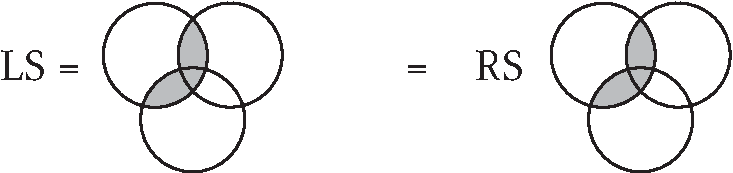
\includegraphics{bilder/kapitel/kap1_Mengen/5.pdf}
\section{Verallgemeinerte Regeln von de Morgan}
\label{sec:VerallgemeinerteRegelnvondeMorgan}
Sind $A_1, A_2 \dots A_n$ alle Teilmengen von $M$ so gilt:
\[\bigcap_{k = 1}^n \overline{A_k} = \bigcup_{k = 1}^n \overline{A_k}\]
\[\bigcup_{k = 1}^n \overline{A_k} = \bigcap_{k = 1}^n \overline{A_k}\]

\section{Aufgaben}
\label{sec:Aufgabe-Mengen-Sportverein}
\subsection{Sportverein}
Von den Mitgliedern eines Sportvereins ist folgendes Bekannt:
\begin{itemize}
	\item Keiner ist zugleich Hand- oder Fu�baller
	\item Alle Eisl�ufer sind Fu�baller
	\item Jeder ist Eisl�ufer oder Skifahrer
\end{itemize}
Zeigen Sie, dass daraus folgt: Jeder Handballspieler ist auch Skifahrer.

L�sung siehe \vref{sec:Loesung-Mengen-Sportverein}.

\subsection{Aufgabe 1}
\label{sec:Aufgabe-Mengen-AufgabeEins}
\renewcommand{\labelenumi}{\alph{enumi})}
\begin{enumerate}
	\item Bestimmen sie $A \backslash B$ und $B \backslash A$ einerseits f�r die Mengen $A=\{1,2,3,4,5\}$ und $B=\{1,2,3\}$ andererseits auch f�r die Mengen $A=\{3,4,5\} $ und $B=\{1,2\}$. Gilt die Aussage $A \backslash B = B \backslash A$? Charakterisieren Sie, wann diese Aussage wahr ist.
	\item Pr�fen Sie die Aussage $A \backslash B = A \cap \overline{B}$ einerseits f�r die Mengen $A=\{1,2,3,4,5\}$ und $B=\{1,2,3\}$, andererseits auch f�r die Mengen $A=\{3,4,5\}$ und $B=\{1,2\}$.
\end{enumerate}

L�sung siehe \vref{sec:Loesung-Mengen-AufgabeEins}.

\subsection{Aufgabe 2}
\label{sec:Aufgabe-Mengen-AufgabeZwei}
Berechnen sie f�r die Teilmenge $D = \{1; 2 ;3 ; \dots; 10\}, S = \{n$ ist Summe zweier Quadrate$\}, P = \{p$ ist Primzahl$\}, U = \{n$ ist ungerade$\}$ und der Grundmenge $\ganzmeng = \{ \dots; -2; -1; 0; 1; 2; \dots \}$ der ganzen Zahlen in die Mengen:
\begin{multicols}{3}
\begin{enumerate}
	\item $P \cap \overline{U}$
	\item $U \cup \overline{U}$
	\item $S \cap D$
	\item $\overline{S} \cap D$
	\item $\left( \overline{S} \cap D \right) \backslash \overline{P}$
	\item $\left( P \cap \overline{U} \right) \times \left( \overline{S} \cap U \right)$
\end{enumerate}
\end{multicols}

L�sung siehe \vref{sec:Loesung-Mengen-AufgabeZwei}.
